\documentclass{subfiles}

\begin{document}
    \marginnote{\textbf{\textit{VL 5}}\\19.04.2023, 08:15}[-1cm]
    \noindent Wir wollen nun die Ergebnisse des vorigen Experimentes festhalten:
    \begin{itemize}
        \item $99.99\si\percent$ der eingestrahlten $\alpha$ Teilchen fliegen geradlinig durch die Au-Folie hindurch. Die Folie ist für die Teilchen also annähernd transparent. 
        \item Der $\alpha$ Teilchenstrom wird leicht aufgefechert. Dies ist mit der erwarteten $e^--\alpha$ Teilchenwechselwirkung vereinbar.
        \item Es wird auch die Rückwertsstreuung (bei den übrigen $0.01\si\percent$ der $\alpha$ Teilchen) beobachtet.
        \item Die zurückgestreuten $\alpha$ Teilchen haben keinen Energieverlust erfahren.
        \item Die Intensität der Rückwertsstreuung ist proportional zur Foliendicke (/-stärke).
        \item Die Winkelverteilung der Zählraten weist die Proportionalität
        \[N(\theta) \propto \frac{1}{\sin(\theta/2)^4}\]
        auf. 
    \end{itemize}
    \subsubsection*{Rutherfordsches Atommodell}\label{Ub:RutherfordModell}\marginnote{$\to$ \hyperref[Ub:AtomEigenschaften]{\faBook}}
    Aus unseren Beobachtungen können wir das \emph{Rutherford-Modell} ableiten:
    \begin{enumerate}[label=(\roman*)]
        \item Atome sind aus Kern und Hülle aufgebaut.
        \item Die Kerne enthalten den Großteil der Atommasse und sind positiv geladen, auf $\approx 40\si{\femto\metre}$ konzentriert.
        \item Die Hüllen enthalten Elektronen, verteilt über das Restvolumen des Atoms.
        \item Das \href{https://de.wikipedia.org/wiki/Coulombsches_Gesetz}{\emph{Coulomb-Gesetz}} behält auf diesen Größenordnungen seine Gültigkeit.
    \end{enumerate}

    \subsubsection*{Die Rutherfordsche Streuformel}
        Wir wollen nun die Streuformel für die Rutherford-Experimente herleiten. Wir betrachten zunächst die Streuung eines $\alpha$ Teilchens auf ein Atom. Die Streuung ist in der Regel sehr klein, sodass wir die Streuung als eine Streuung auf den Atomkern betrachten können. Unser Ziel ist $N(\theta)$. Betrachte das Schema:
        \begin{figure}[H]
            \centering
            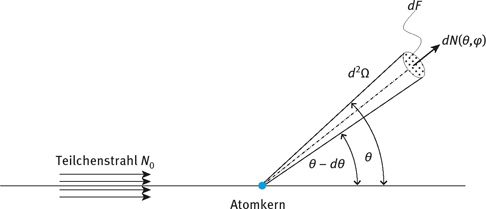
\includegraphics[width=5cm]{Bilddateien/physiko.21.45_9783110445671-fig_001.jpg}
            \caption[short]{Darstellung des schematischen Streuprozesses aus \cite{degruyer:Streuung}.}
            \label{fig:Streuung}
        \end{figure}
        Für die Coulombkraft an einem Ort $r\in\R^3$ erhalten wir zunächst 
        \begin{align*}
            F=\frac{1}{4\pi\epsilon_0}\cdot\frac{2\cdot Z\cdot e^2}{\dabs{r}{2}^3}\cdot r, \label{Ub:CoulombKraftRutherford}\marginnote{$\to$ \hyperref[Ub:AtomEigenschaften]{\faBook}}\tag{$\star$}
        \end{align*}
        wobei $Z\cdot e$ die Ladung des Kerns angibt. Die Kraft wirkt auf das $\alpha$ Teilchen, welches sich mit der Geschwindigkeit $v_0$ auf den Kern zubewegt. 
        Die Kraftaufspaltung in orthogonale und parallele Flugrichtung ergibt
        \[F_\perp=\dabs{F}{2}\cdot\sin(\varphi)\qquad F_\parallel=\dabs{F}{2}\cdot\cos(\varphi).\]
        Für den Drehimpuls erhalten wir in \emph{Zylinderkoordinaten} die Gleichungskette
        \begin{multline*}
            \vec{L}_{r(t)}=\vec{r}(t)\times\vec{p}(t)=\vec{r}(t)\times m\cdot\vec{r}'(t)\\
            =m\cdot \dabs{\vec{r}(t)}{2}^2\cdot\varphi'(t)\cdot(\vec{e}(r(t))\times \vec{e}(\varphi(t)))\\
            =:m\cdot \dabs{\vec{r}(t)}{2}^2\cdot\varphi'(t)\cdot\vec{e_3}.
        \end{multline*} 

        Identifiziere nun $1/r^2=\varphi'(t)/(v_0\cdot b)$ mit $v_0:=\dabs{r'(0)}{2}$ und $b$ als Bahnabstand zur Mittelachse durch den Kern [$\to$ Abb. \ref{fig:Streuung}]. Wir erhalten für das Coulombgesetz 
        \begin{align*}
            F_\perp=\frac{2\cdot q(\text{Ze})^2}{4\pi\epsilon_0}\cdot\frac{\varphi'(t)}{v_0\cdot b}\cdot\sin(\varphi(t))=m\cdot\dabs{r''(t)}{2}
            \label{Ub:OrthKraftRutherford}\tag{$\star$}
        \end{align*}
        und durch Integration 
        \begin{align*}
            b(\theta)=\frac{2\cdot q(\text{Ze})^2}{4\pi\epsilon_0}\cdot\frac{1}{m\cdot v_0^2}\cdot\cot(\frac{\theta}{2}).
            \label{Ub:StreuungBahnabstand}\marginnote{$\to$ \hyperref[Ub:AtomEigenschaften]{\faBook}}\tag{$\star$}
        \end{align*}
        \begin{Aufgabe}
            \nr{} Fülle die Lücken der Rechnung auf. Was kommt beim parallelen Fall heraus?
        \end{Aufgabe}
        Bei unserem Experiment [$\to$ Exp. \ref{exp:Rutherford}] haben wir die \emph{Anzahl der Ereignisse} auf dem Leuchtschirm gemessen. Diese geschahen alle in einem gewissen Raumwinkelbereich $d\Omega$ [$\to$ Abb. \ref{fig:Streuung}], in welchem der Detektor gemessen hat. Wir fragen uns nun, aus welcher Richtung die detektierten Teilchen kommen, was uns auf ein paarweise definiertes Raumelement vor dem Atom bringt: 
        \begin{figure}
            \centering
            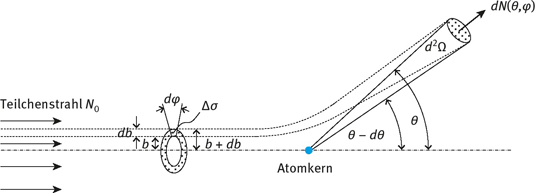
\includegraphics[width=5cm]{Bilddateien/physiko.21.45_9783110445671-fig_002.jpg}
            \caption[short]{Erweiterung der Abbildung \ref{fig:Streuung} um das Ursprungsraumelement \cite{degruyer:Streuung}.}
            \label{fig:StreuungRaumelemente}
        \end{figure}
        Die gemittelte Anzahl der Teilchen $dN$ in diesem Raumelement $d\Omega$ ist augenscheinlich von $db$ ab, sodaß wir auf den schematischen Zusammenhang 
        \begin{align*}
            dN = \emph{Anzahl der }\alpha\emph{ Teilchen}\cdot\frac{dB\cdot \emph{Streuzentrenanzahl}}{\emph{Gesamtfläche}},\label{Ub:dNRutherford}\tag{$\star$}
        \end{align*}
        wobei wir $dB:=\pi\cdot(b^2-(b-db)^2)$ als Trefferfläche und $N_t$ als Streuzentrenanzahl (proportional zur Anzahl der Atome in der Ag-Folie) festhalten. Die Gesamtfläche $F$ ist diejenige der Goldfolie. Daraus ergibt sich
        \[dN = N_\alpha \cdot dB \cdot\frac{N_t}{F}\]
        und \enquote{differenziert} nach $d\Omega$ insgesamt
        \[\frac{dN}{d\Omega} = N_\alpha \cdot\frac{N_t}{F}\cdot\frac{dB}{d\Omega},\]
        wobei wir $dB/d\Omega$ als den \href{https://de.wikipedia.org/wiki/Wirkungsquerschnitt}{\emph{differentiellen Streuquerschnitt}} definieren. 

    \begin{Aufgabe}
        \nr{} Kläre die Bedeutung des angedeuteten Differenzierens. Wie ist der Prozess sauber definierbar?

        \nr{} Verifiziere die alternative Definition $dB:=b\cdot db\cdot d\varphi$. Verifiziere auch $d\Omega=\sin(\theta) \cdot d\theta\cdot d\varphi$. 
    \end{Aufgabe}

    \noindent Die Streuformel für die Rutherford-Experimente lautet nun
    \begin{align}
        \frac{dB}{d\Omega} = \nbra{\frac{1}{4\pi\epsilon_0}\cdot\frac{Z_1\cdot Z_2\cdot e^2}{4\cdot m\cdot v_0^2}}^2 \cdot \frac{1}{\sin(\theta/2)^4}.\label{Ub:RutherfordStreuformel}\marginnote{$\to$ \hyperref[Ub:AtomEigenschaften]{\faBook}}\tag{$\star$}
    \end{align}
    Man kann nun noch $E_0=m\cdot v_0^2$ identifizieren. 

    \paragraph*{Der Kernradius}\label{Ub:starkeKernkraft}
        Für schnelle $\alpha$ Teilchen konnte jedoch experimentell bewiesen werden, daß die Coulombkraft nicht mehr alleinig die Bahn des gestreuten Teilchens beschreiben kann: Es muss eine weitere Wechselwirkung mit dem Atomkern geben, wie sich rausstellen wird die sogenannte \emph{attraktive Kernkraft}.
        \begin{figure}[H]
            \centering
            \begin{subfigure}[b]{0.4\textwidth}
                \centering
                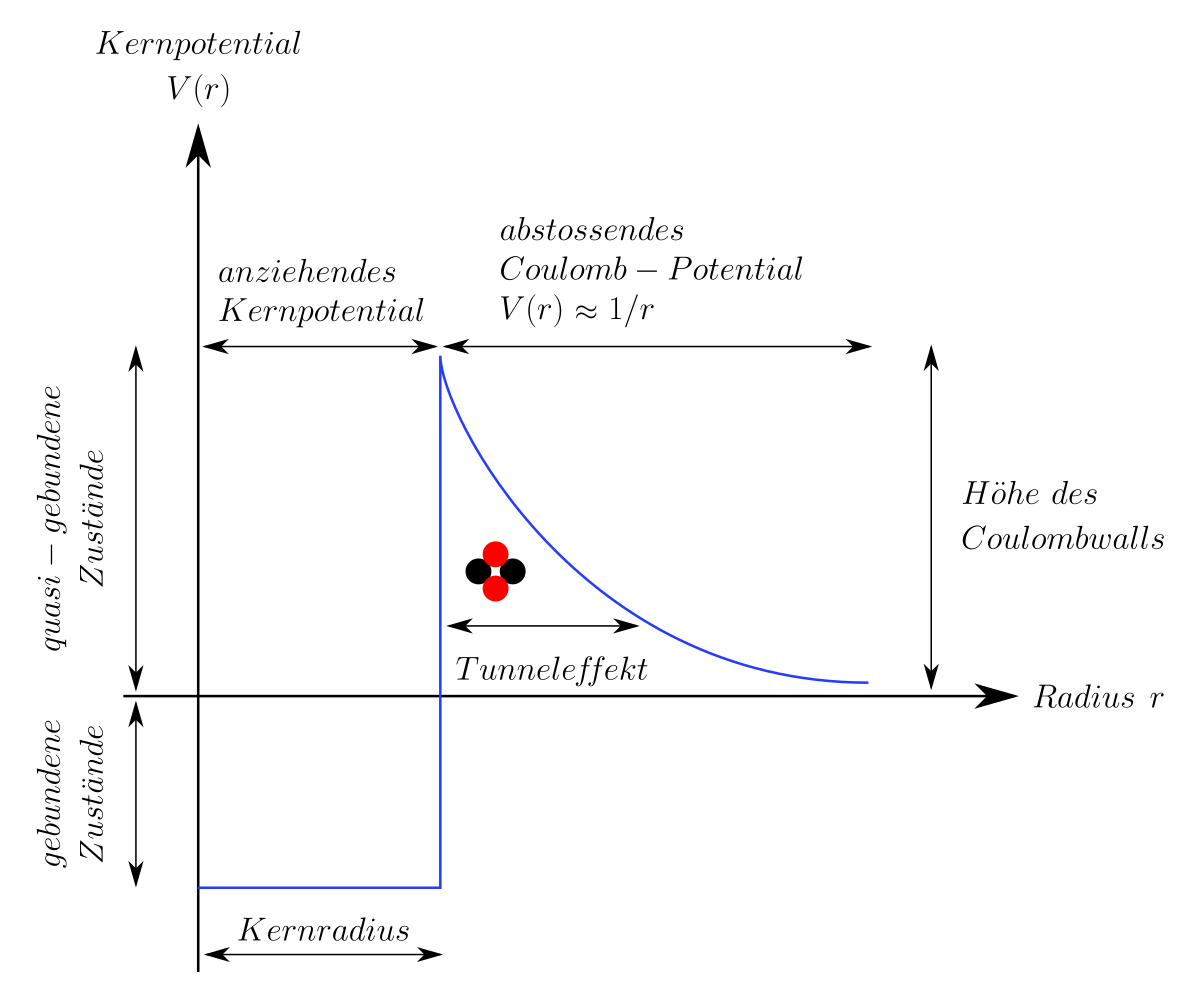
\includegraphics[width=5cm]{Bilddateien/1200px-Tunneleffekt_alpha_zerfall.svg.png}
                \caption{Der Tunnelprozess und die Kernkraft.}
            \end{subfigure}
        \end{figure}

\end{document}